%!TEX root = ../lectures_olympics.tex

\chapter{静电学}

\section{电荷及其微观解释、电荷守恒}

通过一定的操作可以使物体带电,实验中发现物体可能带有两种不同的电荷,分别叫做正电和负电。
通过观察人们发现同种电荷互相排斥,异种电荷互相吸引。
规定和丝绸摩擦后的玻璃棒带正电、毛皮摩擦之后橡胶棒带负电。
宏观带电物体携带电荷数量的多少称为“电荷量”,简称\emph{电量},习惯上用字母$Q$来表示,其单位为\emph{库仑($C$)}。

对物体带电的本质历史上经历了漫长的过程,但对于今天的人们却十分简单。
我们知道所有的宏观物质都是由分子组成,而分子是组成它们的各个原子在空间当中有序排列构成,每个原子无一例外都是由原子核和核外电子所组成。
所有的电子都带负电且电量$e$都相等
\begin{equation}
e\simeq 1.60217733\pow{-19}\unit{C}
\end{equation}
和电子不同的是原子核还有内部结构,它们是由质子和中子共同组成,中子不再电,而质子带正电且电量与电子完全相同\footnote{近代的物理学中认为质子和中子也有其内部结构,但它们的结构不影响它们的电学性质,所以在电学当中不与考虑}。

从这个意义上讲,宏观物体的电量其实是由它内部质子和电子的数量差所决定。
当其内部的电子少于质子时宏观上看就带了负电,反之质子数大于电子数时就带正电。
其电量的绝对值就是两种粒子的数量差与电子电量$e$的乘积。
不带电的物体并不是由于其内部完全没有电荷,而是因为它带有相同数量的质子和电子使得它们的电量彼此抵消而显示为电中性。
但是由于电子电量极其微小且其数目极其庞大,所以通过数粒子数目的方式来确定物体的电量并不可行,实践上还是用库仑来当做电荷的单位。

电荷的一个基本特点是它的守恒,称为\emph{电荷守恒定律}。
它们既不能创造,也不能消灭,它只能从一个物体转移到另一个物体,或从物体的一部分转移到另一部分,在转移的过程中,系统的电荷总数保持不变。
电荷守恒定律在化学当中已经被多次使用,在电学当中它也是分析问题的一个基本要素。
无论是宏观或微观的物理过程,电荷均为严格的守恒量。

\begin{example}
用电荷守恒判断基本粒子的反应产物
\tagged{student}{\vspace*{4cm}}
\begin{taggedblock}{teacher}
\newline
解析:
\end{taggedblock}
\end{example}

\section{静电相互作用力,电场}
\subsection{库仑定律}

前面我们已经提到,带电物体之间同性相斥、异性相吸,通过测量它们之间的作用力人们发现放置于真空当中两个点状电荷之间的作用力正比于它们电量的乘积,反比于它们之间距离的平方,称为\emph{库仑定律}。
如果用$Q_1$,$Q_2$代表两个点电荷的电量,$r$代表它们的距离,则它们之间的作用力的大小
\begin{equation}\label{eqn: coulomb's law}
F = \kc \frac{Q_1Q_2}{r^2},
\end{equation}
其中
\begin{equation}
\kc = 9\pow{9}\unit{N\cdot m^2/C^2}
\end{equation}
$\varepsilon_0$称为真空中的介电常数,其意义在后文当中给出。
当存在有多个点电荷时,一个电荷所受的电力为与其它所有电荷之间由库仑定律所给出力的矢量和。
很容易就会发现库仑定律和万有引力定律有着很多相似的地方,所以在相似的条件下可以借用引力的性质,但也要注意区分它们之间的不同。

\begin{example}
比较两个质子之间的万有引力和库仑力大小的比值。
\tagged{student}{\vspace*{4cm}}
\begin{taggedblock}{teacher}
\newline
解析:
\end{taggedblock}
\end{example}

\begin{example}
著名理论物理学家费曼曾经指出,两个相距一臂之远的人,如果每个人各自有比本身的质子仅多出百分之一的电子,那么两个人之间的排斥力可以举起相当于整个地球的质量。
你能够通过估算给出这一陈述的正确性呢?
\tagged{student}{\vspace*{4cm}}
\begin{taggedblock}{teacher}
\newline
解析:
\end{taggedblock}
\end{example}

\begin{example}
两个带电量均为$Q$点电荷被放置在光滑的水平表面上,它们之间由原长为$l_0$,劲度系数为$k$的弹簧相连接,求平衡时两电荷之间的距离。
\tagged{student}{\vspace*{4cm}}
\begin{taggedblock}{teacher}
\newline
解析:
\end{taggedblock}
\end{example}

\begin{example}
有如图所示的三个点电荷$Q_1$、$Q_2$和$Q_3$位于一条直线上。
其中$Q_1$和$Q_2$之间的距离为$L$,$Q_2$和$Q_3$之间的距离为$2L$,三个点电荷均处于平衡状态,已知$Q_2>0$,求其它两个电荷所携带的电量。
\tagged{student}{\vspace*{4cm}}
\begin{taggedblock}{teacher}
\newline
解析:
\end{taggedblock}
\end{example}

\begin{example}
有一条长度为$l$不可伸长且质量忽略不计的绳,一端系于固定点$O$,另一端挂有一个质量为$m$,电量为$Q$的点电荷$A$。
$O$点正下方$l$处固定有一个等量同种点电荷$B$,求平衡时绳与垂线之间的夹角$\theta$。
\tagged{student}{\vspace*{4cm}}
\begin{taggedblock}{teacher}

解析:
\end{taggedblock}
\end{example}

\begin{example}
原子可以近似地看做是由固定于中心不动的原子核与围绕核转动的电子构成。
已知电子的质量为$m_e$,求当电子沿半径为$r$的圆形轨道匀速转动时的频率。
\tagged{student}{\vspace*{4cm}}
\begin{taggedblock}{teacher}
\newline
解析:
\end{taggedblock}
\end{example}



\subsection{电场、电场强度和电力线}
关于带电体之间的电力是如何传递的很长时间以来都有两种不同的观点。
一种是带电物体之间的作用力是直接作用在两个物体之间,不需要媒质来传递,这就是所谓的超距作用的观点;另一种则是有一种传递电作用的媒质,由于物体带电导致这种媒质产生了某种变化,另一个带电物体感受到了这种变化从而受到了电的作用,这种观点起源于法拉弟关于\emph{电场}的描述。
在早期的电学研究当中两种观点并没有什么不同之处,但随着研究的深入人们发现电相互作用并不是超距的瞬时作用,当一个带电物体的位置发生变化时另一个带电物体并不是立刻察觉这种变化,而是需要一定的时间。
物体之间的电作用似乎是由某种媒质来传递的,但对这种媒质的寻找过程中又遇到了极大的困难,最终的物理告诉我们,电、包括将来要学到的磁相互作用的确能够在真空当中传递,并不需要任何媒质。
但又不是瞬时的超距作用,而是通过一种称之为电场(磁场)的实体对象来传递。
一个带电物体会产生电场,电场有它自身的传递和变化的物理定律,处于一个带电物体产生的电场中的其它带电物体会受到电力的作用。
当产生电场的物体位置发生变化时,它的电场也会随之变化,但这种变化并不是瞬时的而是以光速传递,电场的变化方式将在随后的课程当中详细讨论,在静电学中我们首先来考察电场的基本性质。

设想我们可以拿着一个点电荷在一个带电体周围随意地移动,并且这个点电荷对带电物体的电荷分布的影响能够忽略不计,就称该电荷为\emph{检验电荷}。
一般来说检验电荷在不同位置上所受电力的大小和方向都不同,带电体在空间当中的一点处产生电场的大小和方向用该点处的\emph{电场强度}来描写,电场强度是一个矢量,当把电量为$q$的检验电荷放置于该点时它所受到的电力为
\begin{equation}
\vec{F}=q\vec{E}.
\end{equation}
从定义可以看出某点电场的大小和方向与该点处电荷为$1\unit{C}$的正检验电荷所受电场力完全相同。

电场是一种真空存在着的物理实体,它由带电物体产生,空间当中每一点电场强度的大小和方向被带电体电荷数量及空间分布所决定。
完整地描写电场需要指定空间中各个点的电场强度,在纸上无法完整地表现出来。
比较实用的方法是通过画出一部分点的电场强度来形象地描写整个空间中的电场,正如法拉弟所做的那样。
还可以通过类似于流线的方式将各点的电场强度连起来,称为\emph{电场线}。
一般情况下静电场的电场线为曲线并且具有如下的性质:
\begin{enumerate}
\item 任何一点上的电场强度的方向与电场线的切线方向相同
\item 通过空间当中一点有且只有一条电场线
\item 两条电场线不会相交
\item 电场线密集的地方电场强度较大,反之电场强度较小
\end{enumerate}


很多时候电场强度的定性特征可由电荷分布的对称性所决定,下图为一些典型情况下的电场线的分布情况。


\begin{example}
在长度为$L$的区域内有场强为$E$的匀强电场,其它区域的场强为零。
电子以水平速度$v_0$穿过电场,求电子离开该区域时速度与水平方向的夹角。
因为电子质量极小,忽略电子运动过程中所受的重力。
\tagged{student}{\vspace*{4cm}}
\begin{taggedblock}{teacher}

解析:
\end{taggedblock}
\end{example}



\begin{example}
如图所示,一个质量为$m$,带电量为$q$的点电荷被长度为$l$的不可伸长绳悬挂于固定点上。
整个区域内有场强为$E$的水平方向匀强电场,求平衡时绳与竖直方向的夹角,以及点电荷在平衡位置作微幅摆动的周期。
\begin{flushright}
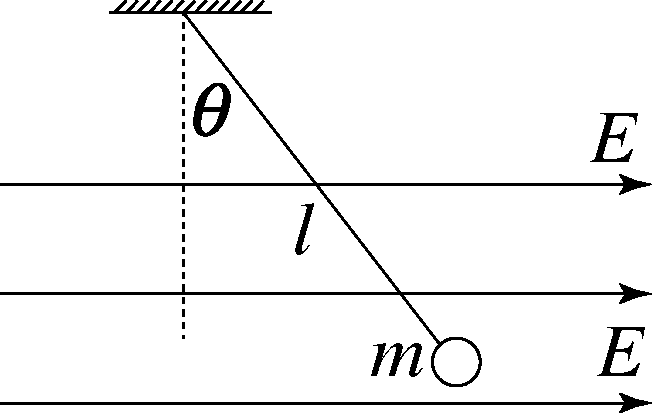
\includegraphics[width=0.3\textwidth]{images/elec-problem-2.pdf}
\end{flushright}
\tagged{student}{\vspace*{2cm}}
\begin{taggedblock}{teacher}

解析:
\end{taggedblock}
\end{example}




\begin{example}
两个电量均为$q$的点电荷距离为$a$,位置如图所示。
求图中$A$、$B$两点的电场强度大小和方向,假设$r_{1,2}\gg a$。
\begin{flushright}
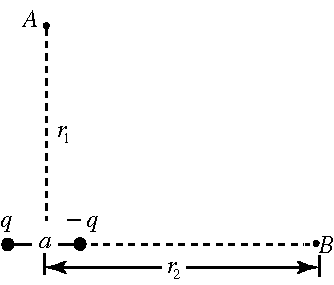
\includegraphics[width=0.4\textwidth]{images/elec-problem-3.pdf}
\end{flushright}
\tagged{student}{\vspace*{1cm}}
\begin{taggedblock}{teacher}

解析:
\end{taggedblock}
\end{example}


\begin{example}
求一个半径为$R$、电量为$Q$的均匀带电圆环在其轴线上任意一点$P$的电场强度,设$P$点到圆心的距离为$d$。
当一个电荷为$-q$,质量为$m$的点电荷被限制在轴线上运动时,求它在平衡位置附近作微幅振动的周期。
\tagged{student}{\vspace*{4cm}}
\begin{taggedblock}{teacher}

解析:
\end{taggedblock}
\end{example}
\subsection{静电场的高斯定律}
电场线和流线有很多的相似之处,沿着电场线似乎像是有某种“东西”在流动。
在液体均匀流动的情况下,做一个垂直于流线的面积为$S$的截面,那么液体的流速与该面积的乘积就代表单位时间时流经该截面液体的体积,或者流量。
与之类似,对于匀强电场同样可以沿垂直于电场线的方向做一个截面,我们将电场强度与截面面积的乘积称做电场的通量,或\emph{电通量}。

对于非均匀的电场和不规则的截面,同样可以定义电通量。
和液体的流量相类比可以看出此时只需要将每个区域的通量相加即可。
如图所示,将截面分割为无限小的区域$\Delta S_i$--后文中将该区域称为面积元--使得截面上通过每个小区域的电场都可近似地看成是匀强电场$E_i$,或者说电场在该区域内的变化量可以忽略不计,一般情况下电场的方向和面积元$\Delta S_i$法线的方向不垂直,而是有夹角$\theta_i$。
这时通过面积元$\Delta S_i$的电通量被定义为
\begin{equation}
\Delta \Phi_i = E_i\Delta S_i\cos\theta_i=\vec{E_i}\cdot\Delta \vec{ S_i},
\end{equation}
这样通过整个截面的电通量就是通过每个截面元电通量的代数和
\begin{equation}
\Phi_S = \sum_{i}\Phi_i = \sum_{i} E_i\Delta S_i\cos\theta_i\footnote{用积分的语言来讲电通量就是电场强度对于给定截面的面积分,$\Phi_S=\int_S \vec{E}\cdot d\vec{S} $}
\end{equation}

静电场的\emph{高斯定律}告诉我们,通过任一闭合曲面的电通量仅与被该曲面包围部分的电量有关:
\begin{equation}
\Phi_C = \frac{1}{\varepsilon_0}\sum_{i\in C}Q_i
\end{equation}
随后的电磁学发展又揭示出,高斯定律不但适用于静电场的情况,对于运动电荷产生的随时间而变的电场同样适用,是电磁学中的一条基本定律。

虽然不可能直接应用高斯定律求解电场的分布,但是当带电体具有某种对称性的话却是可行的。

\begin{example}
根据高斯定律求以下几种情况下给定点的电场强度:

(1)真空中电量为$Q$的点电荷,距离为$r$处

(2)无限长均匀带电的线状带电体,电荷线密度为$\lambda$,与带电线垂线距离为$r$处

(3)无限大的均匀带电平面,电荷面密度为$\sigma$,其表面上方$h$处
\tagged{student}{\vspace*{4cm}}
\begin{taggedblock}{teacher}

解析:
\end{taggedblock}
\end{example}

\begin{example}
根据高斯定律证明:均匀带电球壳内部电场强度为零,外部的电场与其所有电量都集中在球心的点电荷电场完全相同。
\tagged{student}{\vspace*{4cm}}
\begin{taggedblock}{teacher}

解析:
\end{taggedblock}
\end{example}

\begin{example}
求一个半径为$R$,电量为$Q$的均匀带电球体在空间各处产生电场的强度。
\tagged{student}{\vspace*{4cm}}
\begin{taggedblock}{teacher}

解析:
\end{taggedblock}
\end{example}




\begin{example}
有两个带有异种电荷$\pm Q$、面积均为$S$薄板,两板之间的距离$d$远远小于它们的尺寸。
带电板面积为$S$,求两板之间的电场强度以及两板之间的作用力。
\begin{flushright}
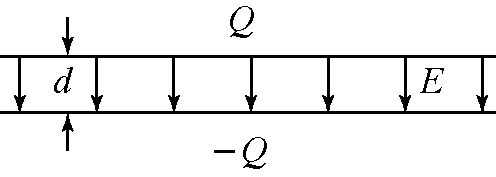
\includegraphics[width=0.3\textwidth]{images/elec-problem-4.pdf}
\end{flushright}
\tagged{student}{\vspace*{3cm}}
\begin{taggedblock}{teacher}

解析:
\end{taggedblock}
\end{example}

\begin{example}
在失重的飞船当中有一个半径为$r$的球形水滴,已知水的表面张力系数为$\sigma_w$。
如果通过一定的手段让它带电,假设水滴所带的电荷均匀分布在它的表面上,由于同种电荷互相排斥,所以当它所带电量超过某一临界值$Q_0$之后水滴必然破裂,求该临界电量的值。
\begin{flushright}
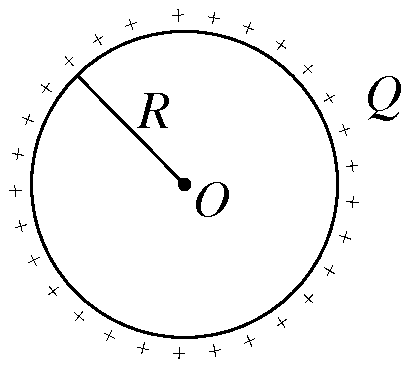
\includegraphics[width=0.3\textwidth]{images/elec-problem-5.pdf}
\end{flushright}
\tagged{student}{\vspace*{4cm}}
\begin{taggedblock}{teacher}

解析:由于表面张力的作用,尽管它处于真空当中水滴内部的压强也不为零,根据表面张力的性质可以求出
\[
p=\frac{2\sigma_w}{r}.
\]
设水滴带电$Q$,均匀分布在它的表面,那么其表面上任意一块小的面积元上的电荷受到的电力等于除了它以外其它所有电荷所产生的电场强度与该表面上的电量的乘积。
根据高斯定律,水滴内部的电场为零,外部电场强度则是
\[
E=\frac{\sigma}{\varepsilon_0}=\frac{Q}{4\pi\varepsilon_0 r^2}
\]
这个电场强度是由所有电荷贡献而得到的。
对于给定面积元上电荷,它所产生的电场实际上有向内和向外两部分,同样依据高斯定律,向内和向外的大小相等,方向相反,均为
\[
E_1 = \frac{1}{2}\frac{\sigma}{\varepsilon_0}
\]
而其它部分贡献的电场强度与它叠加构成了均匀带电球壳的电场,所以其它所有电荷产生的电场
\[
E_2 =  \frac{1}{2}\frac{\sigma}{\varepsilon_0} = \frac{Q}{8\pi\varepsilon_0 r^2}
\]
这样该面积元上电荷所受的电场力的大小则是
\[
F = \frac{Q}{8\pi\varepsilon_0 r^2}\cdot \frac{Q}{4\pi\varepsilon_0 r^2}S = \frac{Q^2}{32\pi^2\varepsilon_0^2r^4}S 
\]
所以由于带电$Q$会产生
\[
\Delta p = \frac{F}{S} = \frac{Q^2}{32\pi^2\varepsilon_0^2r^4}
\]
的向外的附加压强。
简单的分析可知当这个附加压强大于水的表面张力所产生的压强时,水滴将不再可能稳定,而将破裂。
根据这个破裂的条件可得最大允许的带电量为
\[
Q_0=64\sigma_w\pi^2\varepsilon_0^2r^3
\]
\end{taggedblock}
\end{example}

\section{静电能、电势、电势差}
由于带电体之间有库仑力作用,所以当两个带电物体的位置发生变化时或者库仑力会做功,或者需要克服库仑力作功,无论哪种情况下都会有能量的变化。
如果两个物体之间只有库仑力的作用,那么当库仑力作正功时,那么带电物体的速率和动能就会增加,从能量的角度来看就是包含在静电场中某种形式能量转化成物体的动能;反之当需要克服库仑力做功时,机械能就将转化为电场的能量。
和万有引力定律做类比可以看出库仑力是一个保守力,所以在库仑力作用下带电物体运动的机械能守恒。
对于两个电量分别为$Q_1$和$Q_2$的点电荷而言,如果规定当它们相距无限远时的静电势能为零的话,当它们相距$r$时,或者直接计算均可得到它们之间的静电势能或静电能为
\begin{equation}
E = \kc \frac{Q_1Q_2}{ r}
\end{equation}
相对于两个点电荷相距无限远处,同种电荷之间的静电能为正值,反之异种电荷间的静电能为负,这与从库仑力的方向定性判断的结果一致。
如果系统内部包含有多个点电荷,整个系统的静电能则是这些点电荷两两之间静电能的代数和。
对于那些电荷连续分布的带电体,静电能则需要通过将带电体分割成多个可近似看成点电荷的微小部分,通过积分得到电荷连续分布带电系统中所储存的静电能。




\begin{example}
求一个总电量为$Q$,半径为$R$的均匀带电球壳的静电能。
\tagged{student}{\vspace*{4cm}}
\begin{taggedblock}{teacher}

解析:
\end{taggedblock}
\end{example}

当一个带电系统的电荷分布为已知时,空间当中每点的电场强度就被唯一确定。
这时把一个检验电荷缓慢地由无限远处移动到电场当中任意一点电场力的功,或需要克服电场力所需要的机械功也由电场分布唯一确定。
根据电场力的性质,在空间任意一点处检验电荷的静电能正比于它的电量,其比例系数被称做该点的\emph{电势}。
当检验电荷的电量为$q$,当它位于静电场中某点的静电能为$E_p$的话,我们说该点的电势为
\begin{equation}
 U = \frac{E_p}{q}
\end{equation}
它与检验电荷的电量无关,代表着是电场本身的性质。
反过来当空间当中某点的电势$U$为已知时,电量为$q$的带电体在该点的静电能则是
\begin{equation}
E_p = q U
\end{equation}
由于静电能为势能,所以它与该点电荷从无限远处来到该点的路径无关。

简单的计算可以得到,当取无穷远处电势为零时在距离电量为$Q$的点电荷$r$处的电势
\[
U = \frac{1}{4\pi \varepsilon_0}\frac{Q}{r}.
\]
从电场的叠加原理可知证明电势也有类似的叠加原理:多个电荷在某一点处的电势为其单独存在时电势的\emph{代数和},所以当存在多个点电荷$Q_i$、空间中给定$P$点到第$i$个电荷的距离为$r_i$,则$P$点的电势可以写成:
\begin{equation}
U_P = \sum_i \frac{1}{4\pi \varepsilon_0}\frac{Q_i}{r_i}.
\end{equation}
如果电荷是连续分布,那么在计算给定点电势时上式的求和应当换成相应的积分。



\begin{example}
求一个电量为$Q$,半径为$R$的均匀带电球壳产生的电场中各点的电势,取无限远处的电势为零。
\tagged{student}{\vspace*{4cm}}
\begin{taggedblock}{teacher}

解析:
\end{taggedblock}
\end{example}

\begin{example}
有一根无限长的均匀带电直线,电荷线密度为$\lambda$,取距离直线$r_0$处电势为零,求距离直线$r$处的电势。
%\begin{flushright}
%\includegraphics[width = 0.3\textwidth]{images/.pdf} 
%\end{flushright}
\tagged{student}{\vspace*{4cm}}
\begin{taggedblock}{teacher}

解析:
\end{taggedblock}
\end{example}

\begin{example}
证明:均匀带电的半个球壳其开口处的平面上电势处处相等。
%\begin{flushright}
%\includegraphics[width = 0.3\textwidth]{images/.pdf} 
%\end{flushright}
\tagged{student}{\vspace*{4cm}}
\begin{taggedblock}{teacher}

解析:
\end{taggedblock}
\end{example}

\begin{example}
真空中的多个点电荷,第$i$个电荷的电量为$Q_i$,除它自身以外其它点电荷在它所处位置的电势为$U_i'$,求证整个电荷系统的静电能
\[E_p = \frac{1}{2}\sum_i Q_iU_i'.\]

%\begin{flushright}
%\includegraphics[width = 0.3\textwidth]{images/.pdf} 
%\end{flushright}
\tagged{student}{\vspace*{4cm}}
\begin{taggedblock}{teacher}

解析:
\end{taggedblock}
\end{example}

\begin{example}
两个点电荷位于$x$轴上,在它们形成的电场中,若取无限远处的电势为零,则在正$x$轴上各点的电势如图中曲线所示,当$x\rightarrow 0$时电势$U\rightarrow \infty$;当$x\rightarrow \infty$时电势$U\rightarrow 0$;电势为零的点的坐标$x_0$,电势为极小值$-U_0$的点的坐标为$ax_0(a>2)$。
试根据图线提供的信息,确定这两个点电荷所带电荷的符号、电量的大小以及它们在$x$轴上的位置。
\begin{flushright}
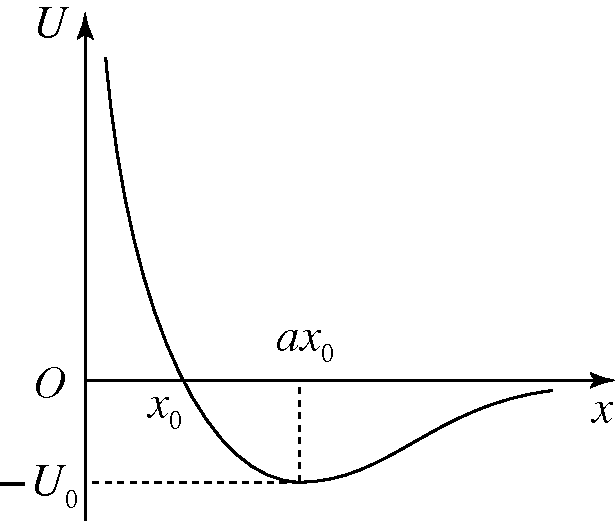
\includegraphics[width=0.4\textwidth]{images/elec-problem-11.pdf}
\end{flushright}
\tagged{student}{\vspace*{4cm}}
\begin{taggedblock}{teacher}

解析:
\end{taggedblock}
\end{example}

因为静电力为保守力所以静电能为势能,和之前遇到的各种势能的情况类似,对于在电场当中运动的带电粒子来说其所处位置的电势能的绝对值并没有意义,而是在某一运动过程前后两点之间势能的差(的负值)才代表电场力对该带电粒子所做的功。
电场当中两点电势的差称为\emph{电势差},假设$A$点的电势为$U_A$,$B$点的电势为$U_B$,则两点之间的电势差
\begin{equation}
U_{AB}=U_B-U_A
\end{equation}
电量为$q$的点电荷从$A$点运动到$B$点静电能的改变量自然就是
\begin{equation}
\Delta E_p = qU_{AB}
\end{equation}
与此同时电场力对该粒子所作的功
\begin{equation}
W_{AB} = -\Delta E_p = -qU_{AB} = -q(U_B-U_A)
\end{equation}
从中可以看出,如果一个正电荷的某个运动过程前后所处位置上电势差大于零,那么它的静电能将会增加,电场力将对它作负功,其它情况请同学们自己分析。

如果已知空间中各点的电场强度,也可推算出给定点的电势。
如图所示,$M$、$N$两点为距离很短的两点,两点间的连线可近似地看成长度为$\Delta l$的直线段,在直线上各点电场强度$\vec{E}$也可认为近似不变。
此时电场强度与$MN$连线方向的夹角为$\theta$,这样两点之间的电势差
\begin{equation}
\Delta U = -E\Delta l \cos\theta
\end{equation}
对于相距较远的$A、B$两点,可以将连接它们的任意一条曲线无限分割成多个小线段,相邻两段之间的电势差由上式给出,而$AB$两点间的电势差则是所有相邻两段电势差的\emph{代数和}。
用数学语言来讲,两点间的电势差可以看成是电场强度沿连接两点任意一条曲线的线积分
\[U_B-U_A = -\int_A^B\vec{E}\cdot d\vec{l}\]

\begin{example}
根据电势差的定义计算以下几种情况下两点之间的电势差:

(1)匀强电场中的$A$、$B$两点,距离为$l$,两点连线与电场线方向夹角为$\theta$。

(2)电荷线密度为$\lambda$的无限长细线外相距分别为$r_{1,2}$的两点$A$和$B$。

(3)电荷体密度为$ \rho$的均匀带电球体内部与球心相距$r_{1,2}$的两点。

\tagged{student}{\vspace*{4cm}}
\begin{taggedblock}{teacher}

解析:
\end{taggedblock}
\end{example}

\begin{example}
如图所示的两个带电板中间各有一个小孔可以让电子通过。
为了使电子在通过板之后的动能增加,需要$U_A\underline{\qquad}U_B$,如果两板之间的电势差为$U$,距离为$d$,电子的初速度为$v_0$,忽略重力求电子通过两板所需要的时间。
\begin{flushright}
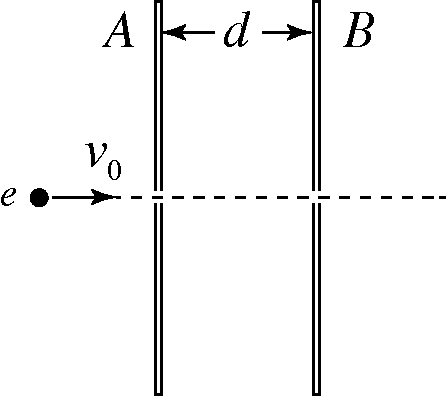
\includegraphics[width=0.3\textwidth]{images/elec-problem-6.pdf}
\end{flushright}
\tagged{student}{\vspace*{1cm}}
\begin{taggedblock}{teacher}

解析:
\end{taggedblock}
\end{example}




\begin{example}
两块竖直放置的平行金属大平板$A$、$B$,相距$d$,两极间的电势差为$U$。
一个带正电的质点从两板间的$M$点开始以竖直向上的初速度$v_0$运动,当它到达电场中某点$N$时,速度变为水平方向,大小仍为$v_0$,如图所示。求两点间的电势差。(忽略带电质点对金属板上电荷分布的影响)
\begin{flushright}
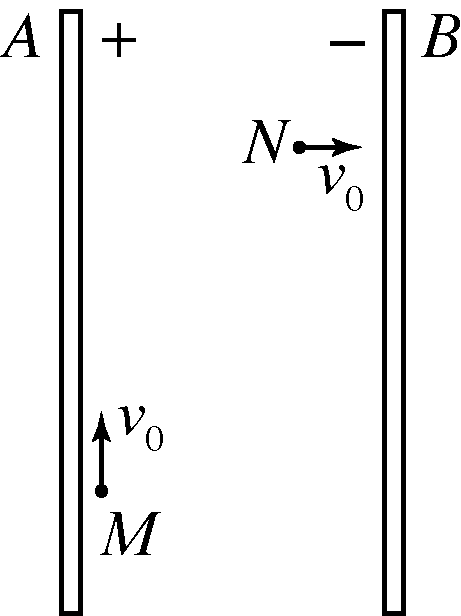
\includegraphics[width=0.2\textwidth]{images/elec-problem-1.pdf}
\end{flushright}
\tagged{student}{\vspace*{2cm}}
\begin{taggedblock}{teacher}

解析:
\end{taggedblock}
\end{example}

\begin{example}
如图所示,在水平光滑的绝缘桌面上有三个带正电的质点1、2、3,位于边长为$L$的等边三角形的三个顶点处,$C$为三角形的中心。
三个质点的质量皆为$m$,带电量均为$q$。
质点1、3之间和2、3之间用绝缘的轻而细的刚性杆相连,在3的连接处为无摩擦的铰链。
已知开始时三个质点的速度为零,在此后运动过程中,当质点3运动到$C$处时,其速度为多少?
\begin{flushright}
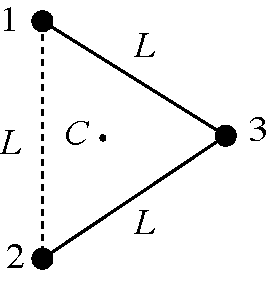
\includegraphics[width=0.2\textwidth]{images/elec-problem-10.pdf}
\end{flushright}
\tagged{student}{\vspace*{4cm}}
\begin{taggedblock}{teacher}

解析:
\end{taggedblock}
\end{example}

\begin{example}
最粗略的近似下质子可以看成是半径为$r_p$的均匀带电球,其半径至少小于$10^{-15}\unit{m}$。
有两个质子以相同的速率相向运动,求它们能够相撞所需要的最小能量。
\begin{flushright}
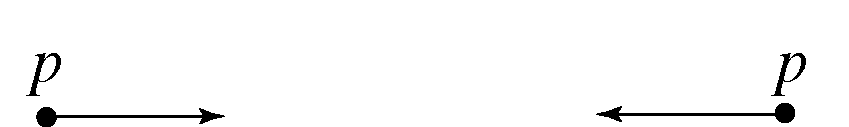
\includegraphics[width=0.4\textwidth]{images/elec-problem-9.pdf}
\end{flushright}
\tagged{student}{\vspace*{2cm}}
\begin{taggedblock}{teacher}

解析:
\end{taggedblock}
\end{example}

\begin{example}
有两个相距为$2L$,电量均为$Q>0$的固定点电荷$A$、$B$,现有另外一个电量为$q$,正负未知的点电荷$C$被限制在通过$AB$连线中点,夹角为$\theta$的直线$MN$上运动。
求$C$可能的平衡位置和在平衡位置附近作微幅振动的周期。
\begin{flushright}
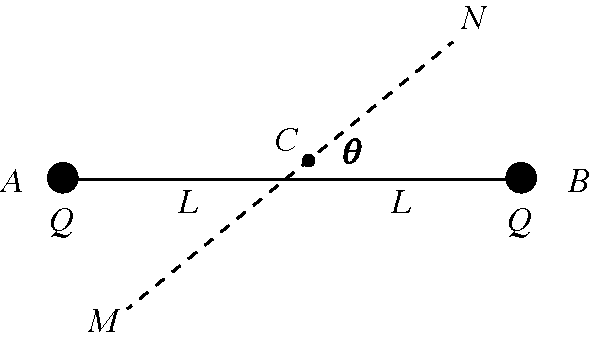
\includegraphics[width=0.4\textwidth]{images/elec-problem-7.pdf}
\end{flushright}
\tagged{student}{\vspace*{4cm}}
\begin{taggedblock}{teacher}

解析:
\end{taggedblock}
\end{example}

\begin{example}
有一个固定放置的半径为$R$的均匀带电球体,$O$为其球心。
当把无限远处的电势为零时,球表面处的电势$U=1000\unit{V}$。
在离球心很远处有一个质子,以$E = 2000\unit{eV}$的动能射向带电球,瞄准参数为$b$,其意义如图所示。
要使质子能够与球体相撞,求$b$的最大值。
\begin{flushright}
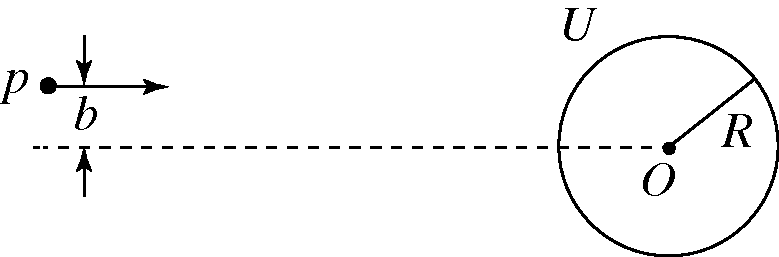
\includegraphics[width=0.4\textwidth]{images/elec-problem-8.pdf}
\end{flushright}
\tagged{student}{\vspace*{4cm}}
\begin{taggedblock}{teacher}

解析:
\end{taggedblock}
\end{example}

电势和电场在描写静电场分布方面是等价的,它们都是由电荷的分布所唯一决定,所以它们之间也必然有联系。
前面已经看到,将各点的电场连起来就构成了电场线。
对于电势来说,它是一个标量,所以我们有机会在电场当中可以确定两点之间电势是否相同。
很容易想到的是与空间当中一个给定点的电势相同的所有点一般来说会构成一个曲面,静电学当中称其为通过该给定点的\emph{等势面}。
通过空间中一点有且只有一个等势面,它的电势就是该等势面的电势,对应于两个不同电势的等势面必然不会相交,两个面的电势之差就是两个等势面的电势差。
带电粒子从一个等势面上任意一点运动到第二个等势面上任意一点电势能的变化均相同。
将电场线和等势面放在一起还能够发现,电场当中任意一点处的电场线和通过该点的等势面均垂直,并且电场线指向电势降低的一侧。
电场线和等势面的这一特点的一个直接推论就是如果空间当中某一区域内部的电势均相同,该区域内部的电场强度必然为零。

当所有带电体的位置和电荷分布为已知时,空间中各点的电势也就被唯一确定,建立平面直角坐标系$(x,y,z)$,电势作为坐标的函数用$U(x,y,z)$表示。
在给定点上电场强度由矢量$(E_x,E_y,E_z)$给出,根据电势和电场强度的关系可知
\begin{equation}
E_x = \frac{\partial U}{\partial x},\qquad E_y = \frac{\partial U}{\partial y},\qquad E_z = \frac{\partial U}{\partial z},
\end{equation}
从中也能够很容易得到,电势处处相等则必然场强为零。
另外当电势在某一个具体的方向上保持不变,则在这个方向上也没有电场强度的分量。
如果电势沿某一方向均匀增加,则意味着有一个沿该方向的匀强电场,电场强度由是单位距离上电势的减少量。

\begin{example}
几种对称情况下的等势面和电场线,以及定量的关系 
\tagged{student}{\vspace*{4cm}}
\begin{taggedblock}{teacher}

解析:
\end{taggedblock}
\end{example}

\begin{example}
几种典型的非对称情况下的等势面和电场线
\tagged{student}{\vspace*{4cm}}
\begin{taggedblock}{teacher}

解析:
\end{taggedblock}
\end{example}

\begin{example}
一些定性的判断
\tagged{student}{\vspace*{4cm}}
\begin{taggedblock}{teacher}

解析:
\end{taggedblock}
\end{example}



\section{电场中的导体}

前面我们讨论了很多规则分布电荷产生的静电场的性质,从中可以看出当电荷分布为已知时在一定情况下可以得到全部空间中电场线的分布情况,等价地电势分布也自然可以得到。
但实际上电荷的分布并不总是能够在一开始就被完全确定,有一类电荷是由人为地使体积很小的物体带电并主动地放置在空间中某处的,这种带电体可以看做点电荷,这种情况下自然该电荷的电量和位置就可以完全确定。
但是当把该电荷放在给定点上时,它所产生的电场就会与其它物质当中的带电物质,也就是原子核和电子之间有静电作用。
有可能物质当中的带电粒子会在电场力作用下做运动,从而改变其中的电荷分布,这种现象称为\emph{静电感应}。
由静电感应所产生的电场并不是可以预先给定的,依赖于外部电荷的大小和位置,这就为电场的分析带来了一定程度的复杂性。
在电磁学中有两类性质迥异的物质,依据组成它们的分子、原子性质的不同分别是\emph{导体(electrical conductor)}和\emph{绝缘体(insulator)}。

金属是最典型导体的例子,构成金属物质的原子核对一部分电子的束缚很弱,这些电子脱离原子而形成自由电子,在外部电场力作用下这些电子能够运动。
其实不仅是金属,只要物质当中存在有可以自由运动的带电粒子,都是导体。
例如电解质(electrolytes)也是导体的一种,在电解质中承担导电任务不是自由电子,而是离子;等离子体(plasma)则是由等量的正负电荷构成的电中性的混合物,两种电荷均可导电。
在特殊条件下还会存在所谓的超导体(superconductor),超导体的电阻率为零,超导体中承担导电任务的不是普通的电子,而是由两个电子捆绑而成的库珀电子对,在晶格中运动完全不受阻力。
总得来说,无论以何种方式提供了可自由运动的带电粒子的物质都是导体。

而绝缘体则不同,其内部没有自由运动的电子,但是在外电场作用下电子和原子核由于电荷不同从而受到不同方向的外力;形象地看原子就会外电场“拉开”形成\emph{电偶极子},最终绝缘体内部的电场是由外电场和这些电偶极子电场的叠加,绝缘体也被称做\emph{电介质}。
本节首先来讨论当电场当中存在有导体的情况,下一节则着重关注存在电介质的问题。
需要特别强调的是绝缘体和导体的区别并不是绝对的,导体在特殊条件下能够转化为绝缘体,绝缘体也能够转化为导体。

从导体的性质通过简单的分析可知,处于静电平衡的导体内部的电场必然为零,否则带电粒子依然会在电场力作用下运动,直到导体的电荷分布和外电场叠加以后的总电场在导体内部处处为零为止。
以此出发还能够得到以下推论:
\begin{enumerate}
\item 静电平衡的整个导体内部的电势均相等,导体是一个等势体,表面是一个等势面。
根据导体所处环境的不同其电势或者由外部电荷间接决定,或者直接由外接电源给出。
\item 
导体表面外部的电场垂直于表面,其大小由面电荷分布给出。
\item 静电平衡状态下的导体空腔内表面总电荷必然与处于空腔内部的电荷相等,如果内部总电荷为零那么所有电荷全部位于其外表面,导体空腔内部电场处处为零,这个现象称做\emph{静电屏蔽}。
\end{enumerate}


%%%%%%%%%%%%%%%%%%%%%%%%%%%%%%%%%%
\begin{example}
将两个相距很远,半径分别为$R_1$、$R_2$的导体球由导线连接,求静电平衡以后两导体球上电量、电荷面密度的比值。
\tagged{student}{\vspace*{4cm}}
\begin{taggedblock}{teacher}

解析:因为两球相距很远,所以它们所带的电荷对对方的电势贡献可以忽略不计;又因为它们由导线连接,所以两者的电势相等。
设平衡后带电量分别为$Q_{1,2}$,则有
\[
\frac{1}{4\pi \varepsilon_0}\frac{Q_1}{R_1} = \frac{1}{4\pi \varepsilon_0}\frac{Q_2}{R_2},\qquad  \frac{Q_1}{R_1} = \frac{Q_2}{R_2}
\]
而且两者均为均匀带电,所以
\[
\frac{ \sigma_1 4 \pi R_1^2}{R_1} = \frac{ \sigma_2 4 \pi R_2^2}{R_2},\qquad \sigma_1R_1 = \sigma_2R_2 
\]
可见半径越小的球电荷面密度越大,其表面附近的电场强度则越大,这个结果是尖端放电现象的原因。
\end{taggedblock}
\end{example}
%%%%%%%%%%%%%%%%%%%%%%%%%%

%%%%%%%%%%%%%%%%%
\begin{example}

在内、外半径分别为$R_1$,$R_2$的导体球壳内,有一个半径为$r$的导体小球,小球与球壳同心,让小球与球壳分别带上电荷量$q$和$Q$。
试求:

(1)小球的电势$V_r$,球壳内、外表面的电势。

(2)小球与球壳的电势差。

(3)若球壳接地,再求小球与球壳的电势差。
\begin{flushright}
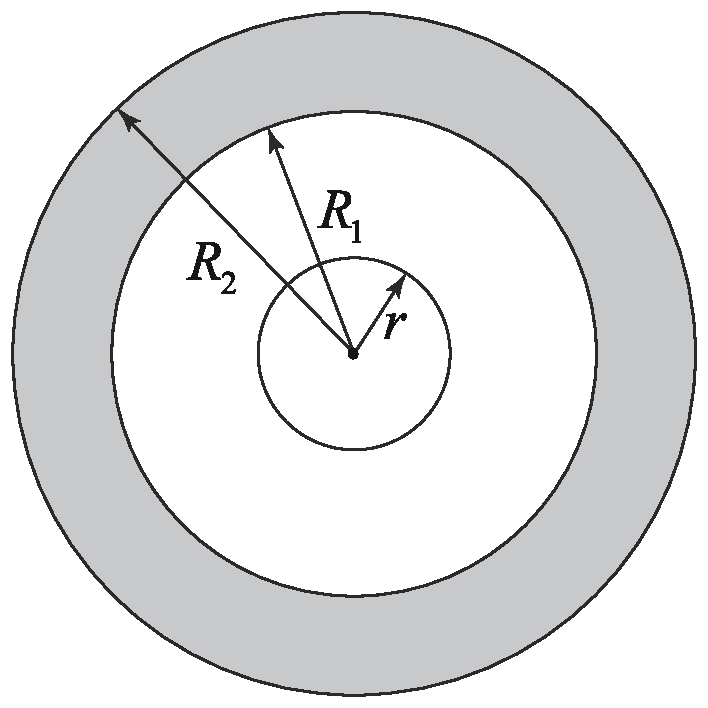
\includegraphics[width = 0.3\textwidth]{images/elec-problem-13.pdf} 
\end{flushright}
\tagged{student}{\vspace*{1cm}}
\begin{taggedblock}{teacher}

解析:根据导体的性质可知,静电平衡以后大球内表面电荷$-q$,电荷守恒则要求外表面电荷$Q+q$,整个系统球对称,所有面上电荷都是均匀分布。
这样小球的电势
\[
U_r = \kc \left(\frac{q}{r}-\frac{q}{R_1}+\frac{q+Q}{R_2}\right)
\]
同样的道理可以算出大球内、外表面的电势
\[
U_{R_1} = \kc \left(\frac{q}{R_1}-\frac{q}{R_1}+\frac{q+Q}{R_2}\right) = \kc\frac{q+Q}{R_2},U_{R_2} = \kc \left(\frac{q}{R_2}-\frac{q}{R_2}+\frac{q+Q}{R_2}\right) = \kc\frac{q+Q}{R_2},
\]
肯定地,它们是等势体。
将两个电势相减就是两部分的电势差:
\[
\Delta U = \frac{q}{4\pi\varepsilon_0}\left(\frac{1}{r}-\frac{q}{R_1}\right),
\]
最后球壳接地后它的电势必然为零,但影响的只有外表面的电荷,所以电势差和前一问完全相同。
\end{taggedblock}
\end{example}
%%%%%%%%%%%%%%%%%%%%%%




%%%%%%%%%%%%%%%%%
\begin{example}
已知:使一原来不带电的导体小球与一带电荷为$Q$导体大球接触,分开之后小球获得电荷量$q$。
今让小球与大球反复接触,在每次分开后,都给大球补充电荷,使其电荷量恢复到原来的值$Q$。
求小球可能获得的最大电量。

\tagged{student}{\vspace*{4cm}}
\begin{taggedblock}{teacher}

解析:每次接触以后两者成为等势体,电量分配之比则是
\[
\frac{q}{Q-q},
\]
这样无数次以后两者之间再无电荷交换,则有
\[
\frac{q_f}{Q} = \frac{q}{Q-q},\qquad q_f = \frac{qQ}{Q-q}
\]
\end{taggedblock}
\end{example}
%%%%%%%%%%%%%%%%%%%%%%








\begin{example}
如图所示,O为半径等于$R$的原来不带电的导体球的球心,$O_1$、$O_2$、$O_3$为位于球内的三个半径皆为$r$的球形空腔的球心,它们与$O$共面,已知$\overline{OO_1}=\overline{OO_2}=\overline{OO_3}=\frac{R}{2}$。
在$OO_1、OO_2$的连线上距离$O_1、O_2$为$r/2$的$P_1、P_2$点处分别放置电量为$q_1$和$q_2$的线度很小的导体(视为点电荷),在$O_3$处放置一带电量为$q_3$的点电荷,设法使$q_1、q_2$和$q_3$固定不动。
在导体球外的$P$点放一个电量为$Q$的点电荷,$P$点与$O_1、O_2、O_3$共面,们于$\overline{O_3O}$的延长线上,到$O$的距离$\overline{OP}=2R$。

(1) 求$q_3$的电势能

(2) 将带有电量$q_1、q_2$的小导体释放,当重新达到静电平衡时,各表面上的电荷分布有何变化?
此时$q_3$的电势能为多少?
\begin{flushright}
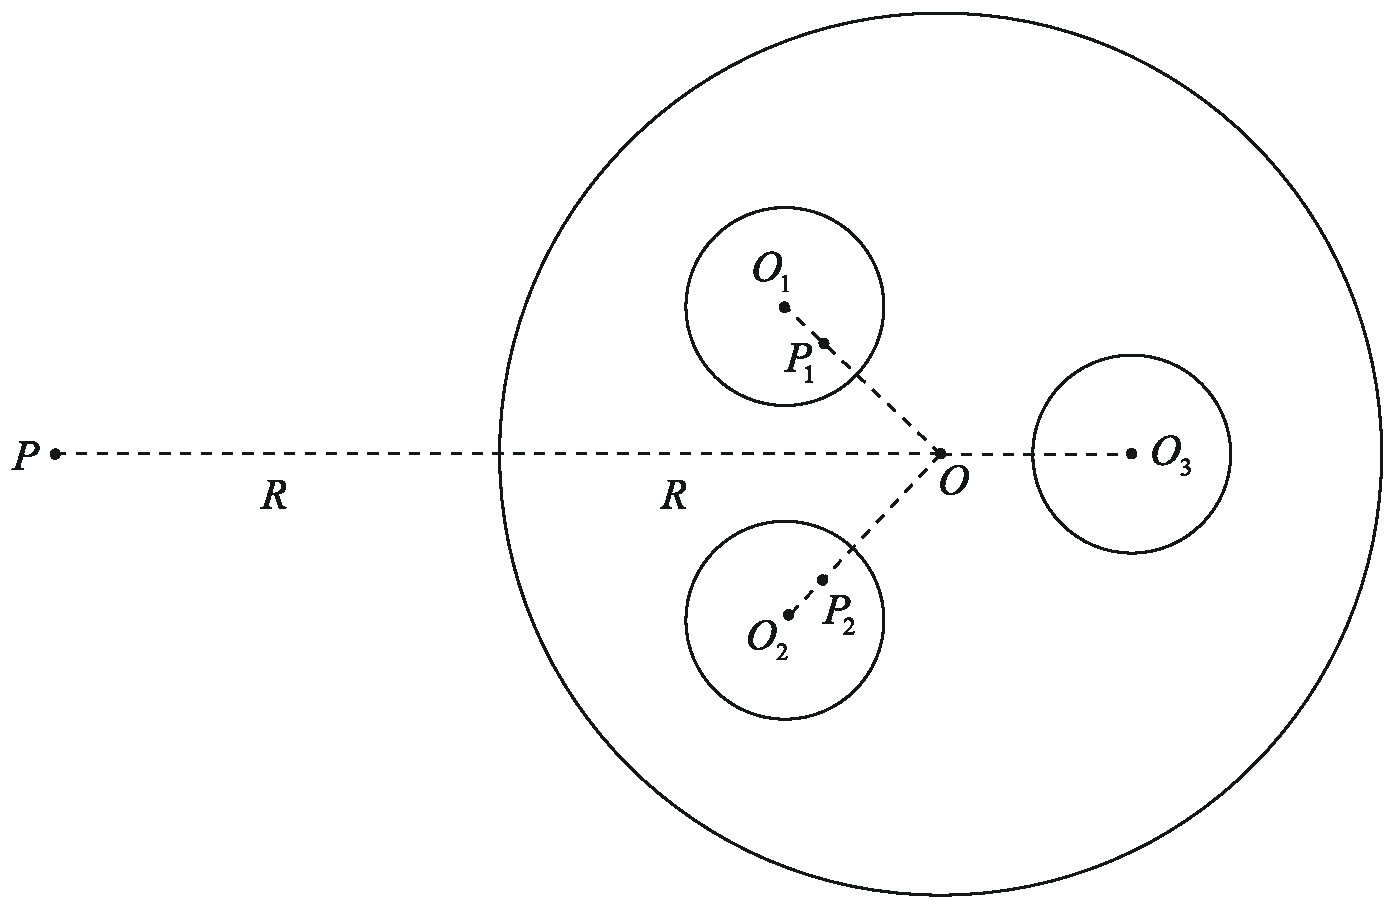
\includegraphics[width = 0.4\textwidth]{images/elec-problem-12.pdf} 
\end{flushright}
\tagged{student}{\vspace*{4cm}}
\begin{taggedblock}{teacher}

解析:
\end{taggedblock}
\end{example}

\subsection{电场的唯一性定理,电像法}


\begin{example}
将一个电量为$Q$的点电荷$A$被放置于接地的无限大金属板距离为$d$点处,试求感应电荷对它的作用力、金属板右侧电势分布的表达式和板上感应电荷的分布。
\begin{flushright}
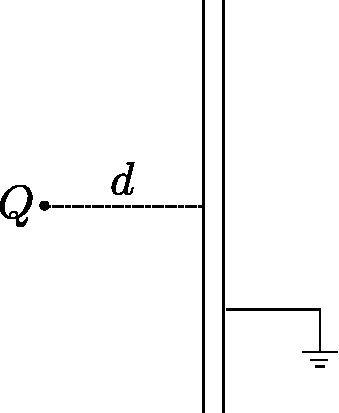
\includegraphics[height = 4cm]{images/elec-img-problem1.pdf} 
\end{flushright}
\tagged{student}{\vspace*{0cm}}
\begin{taggedblock}{teacher}

解析:本题为电像法的一个简单应用,如果在金属板右侧镜向位置处有一个等量异种的电荷的话,它们的垂直平分面就将是一个电势为零的等势面,这和接地导体的边界条件完全一致,所以在整个左侧区域在外电荷Q和感应电荷共同作用下的电场分布与Q和镜向电荷共同作用的电场分布一致。
所以Q和金属板的作用力和作用能
\[F = \kc\frac{Q^2}{(2d)^2},\qquad E_p = -\kc\frac{Q^2}{2d}\]
\end{taggedblock}
\end{example}




\begin{example}
试从数学上证明距离空间当中给定两点距离之比为常数的所有点构成一个球体。
并以此出发根据静电场的唯一性证明如图所示的,一个电量为$q$的点电荷$A$放在一个半径为$R$的接地金属球周围,它将在金属球表面产生感应电荷在金属球外部的静电效应与一个位于球心与该电荷连线上某处$B$带给定电量的电荷的电效应完全一致。
并给出该点荷(电像)的电量$q'$和它到球心的距离$d'$,并进一步以此确定感应电荷对电荷$q$的作用力。
\begin{flushright}
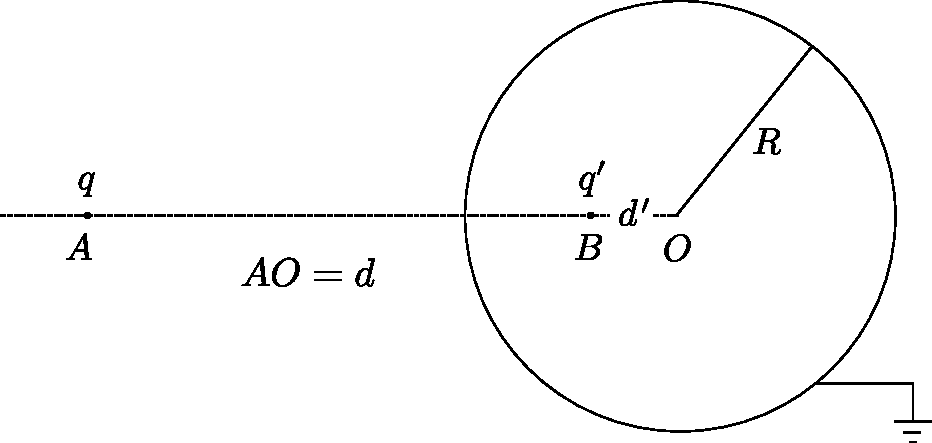
\includegraphics[width = 0.4\textwidth]{static-elec/charge-image.pdf} 
\end{flushright}


\tagged{student}{\vspace*{3cm}}
\begin{taggedblock}{teacher}


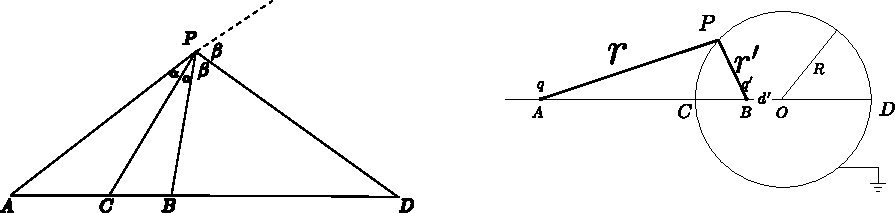
\includegraphics[width=0.9\textwidth]{static-elec/charge-image-solution.pdf} 

解析:几何证明:假设两点分别为$A$和$B$,图中的$P$点到两点之间的距离之比为给定值$k$,在AB的连线上选取两点C和D,它们分别满足
\[
\frac{AC}{CB}=k,\qquad \frac{AD}{BC}=k
\]
这样根据几何关系,在三角形ACP和CPB当中使用两次正弦定理可以判断出角APC等于角CPB,所以CP为角APB的角平分线。
同样的道理可知DP为三角形ABP外角的角平分线,这样可知图中$\alpha+\beta=\pi/2$,对所有的P点均满足,所以P均位于以CD为直径的圆上,对应于立体图形则P全部位于以CD为直径的球体上。

这样就有机会在球体内部找到一个镜像电荷使得接地金属球表面电势处处为零。
因为在球面上任意一点P上A和B的电势之和
\[
U=\kc\frac{q}{r}+\kc\frac{q'}{r'}
\]
如果取$q'$电量与$q$相反,那么存在有一个球使得球面上的电势处处为零:
\[
\frac{q}{r}=\frac{-q'}{r'},\qquad \frac{r}{r'}=-\frac{q}{q'}
\]
当这一点清楚了以后,对于给定的接地金属球,只需要用其上面任意两点的电势为零就可以确定镜像电荷的大小和位置,它和外部电荷A一起一定能够使得整个金属球上的电势为零。
简单起见取图中的C、D两点,它们位于球体表面在A和球心连线的方向上,它们的电势为零的条件为
\[ \frac{q}{d-R}+\frac{q'}{R-d'}=0,\qquad \frac{q}{d+R}+\frac{q'}{R+d'}=0 \]
联立以上两式可以解出:
\[  d'=\frac{R^2}{d},\qquad q' = -q\frac{R}{d} \]

有了电像的电量和位置以后剩下的问题就简单了,外电荷$A$与感应电荷的作用力与$A$与镜像电荷的静电力完全一致:
\[F = -\kc \frac{q q\frac{R}{d}}{(d-\frac{R^2}{d})^2} =-\kc  \frac{q^2 Rd}{(d^2-R^2)^2}, \]
异性相吸,同理静电能
\[E_p = -\kc\frac{q^2R}{d^2-R^2}\]
从中可以看出电荷A和感应电荷的相互作用与它与球心距离的关系。


\end{taggedblock}
\end{example}



\begin{example}
求一个带电量为$Q$,半径为$R$的导体球与另一个带电量为$q$,与球心相距$d$的点电荷$B$之间的静电力的大小。
\tagged{student}{\vspace*{4cm}}
\begin{taggedblock}{teacher}

解析:电像法的一个应用,导体的感应电荷在球外部的电场与由$B$的镜像电荷$q' = - \frac{R}{d}q$与均匀分布在导体表面,大小为$Q-q' = Q + \frac{R}{d}q$电荷共同决定的电场完全相同。
取排斥力方向为正,两者之间的作用力
\[
F = \kc \frac{(Q+\frac{R}{d}q)q}{d^2}-\kc \frac{ \frac{R}{d}q^2}{(d- \frac{R^2}{d})^2},
\]
将上式化简就可得两者之间的作用力,正则是排斥力,反之是吸引力。
\end{taggedblock}
\end{example}


%%%%%%%%%%%%%%%%%%%%%%%%%%%%%%%%%%
\begin{example}
内、外半径分别为$R_1$和$R_2$的同心导体球内部有一个电量为$q$,与球心相距$a<R_1$的点电荷,求空间各处的电势。
\begin{flushright}
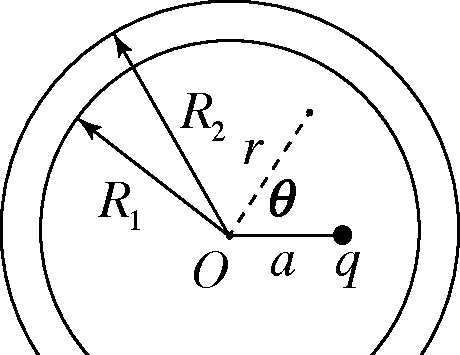
\includegraphics[width=0.4\textwidth]{images/elec-problem-14.pdf}
\end{flushright}
\tagged{student}{\vspace*{4cm}}
\begin{taggedblock}{teacher}

解析:
\end{taggedblock}
\end{example}
%%%%%%%%%%%%%%%%%%%%%%%%%%

\begin{example}
电势为零电像法中的摆动问题
\tagged{student}{\vspace*{4cm}}
\begin{taggedblock}{teacher}

解析:
\end{taggedblock}
\end{example}






\section{电介质、电容}

考虑一个由多个导体构成的系统,除了一个以外其余导体全部接地,这时当那个不接地的导体带电量为$Q$时,由静电场的规律可知它的电势将正比于它的电量。
将这个比例系数称为该系统的\emph{电容},用$C$来表示:
\begin{equation}
C = \frac{Q}{U}.
\end{equation}\label{eqn: static-elec-孤立导体的电容}
简单的观察可以发现电容与所带电量无关,但与所有导体的形状与位置密切相关。
考虑一个最简单的情况,除了一个位于真空、半径为$R$的孤立导体球,根据前面的知识当取无限远处电势为零时它的电势
\[
U = \frac{1}{4 \pi \varepsilon_0}\frac{Q}{r},
\]
根据电容的定义,它的电容
\begin{equation}
C = \frac{Q}{U} = 4 \pi \varepsilon_0 R.
\end{equation}
同样的道理,对于如图\ref{fig: 平行板电容器}所示的双极电容,或平行板电容器,当相对两极板分别带有等量异种电荷$Q$,保持两板之间为真空,而知为$S$且相距$d$时,根据高斯定律两板之间存在有大小$E = \frac{Q}{ \varepsilon_0 S}$的匀强电场,这样两板之间的电势差为
\[
\Delta U = E d = \frac{Qd}{ \varepsilon_0 S},
\]
根据电容的定义也可得出给定参数的平行板电容器的电容
\begin{equation}
C = \frac{Q}{U} = \varepsilon \frac{S}{d}.
\end{equation}
同样的道理可以得到其它情况下的电容。例如


\begin{example}
忽略边缘效应,求长度为$L$,内外半径分别为$R_1$、$R_2$的同心圆柱导体系统的电容
\tagged{student}{\vspace*{4cm}}
\begin{taggedblock}{teacher}

解析:
\end{taggedblock}
\end{example}

\begin{example}
求由两个半径分别为$R_1$、$R_2$,中间为真空的同心导体球壳构成体系的电容。
\tagged{student}{\vspace*{4cm}}
\begin{taggedblock}{teacher}

解析:
\end{taggedblock}
\end{example}

%%%%%%%%%%%%%%%%%%%%%%%%%%%%%%%%%%
\begin{example}
一个平行板电容器两极板面积均为$S$,相距$d$,中间为真空且忽略边缘效应。
当它带电为$Q$时,求电容器储存的能量、两板之间的作用力
\tagged{student}{\vspace*{4cm}}
\begin{taggedblock}{teacher}

解析:
\end{taggedblock}
\end{example}
%%%%%%%%%%%%%%%%%%%%%%%%%%

\begin{example}
两平行放置很大的金属薄板$A$和$B$,面积均为$S$,间距为$d\ll\sqrt{S}$,已知$A$板带电$+Q_1$,$B$板带净电量$+Q_2<Q_1$,求:

1. 两板内、外表面的电量分别为多少

2. 空间各处的场强

3. 两板之间的电势差。
\tagged{student}{\vspace*{4cm}}
\begin{taggedblock}{teacher}

解析:
\end{taggedblock}
\end{example}

%%%%%%%%%%%%%%%%%%%%%%%%%%%%%%%%%%
\begin{example}
$A、B、C$是三块平行金属板,面积均为$200\unit{cm^2}$,$A、B$两板相距$4.0\unit{mm}$、$A、C$两板相距$2.0\unit{mm}$,$B、C$两板都接地,如图所示。
设$A$板带正电$3.0\pow{-7}\unit{C}$,不计边缘效应,求$B$、$C$两板上的感应电荷及$A$板的电势。
\tagged{student}{\vspace*{4cm}}
\begin{taggedblock}{teacher}

解析:
\end{taggedblock}
\end{example}
%%%%%%%%%%%%%%%%%%%%%%%%%%

%%%%%%%%%%%%%%%%%
\begin{example}

静电加速器,其高压电极外面都有一接地的金属罩,罩内充有一定压强的气体。
设电极是一个金属球,接地金属罩是一同心金属薄球壳,如图所示,仪器工作时电极与金属罩之间的电势差为$U_0$。

1. 若$R_1$已给定,则在理想情况下$R_2$取何值,电极处的场强有极小值;

2. 在实际情况中往往适当选择$R_1/R_2$之值,使电极处的场强为上述最小值的若干倍,但仍低于击穿场强。
求当电极场强为上述最小值4倍时,$R_1/R_2$应选的值。
\begin{flushright}
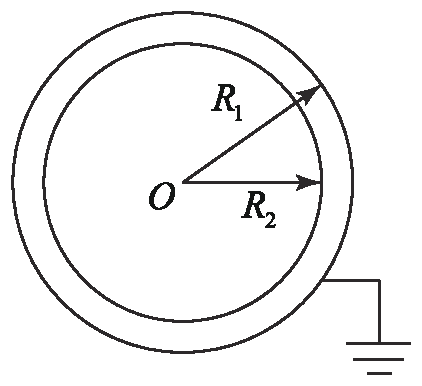
\includegraphics[width = 0.3\textwidth]{images/elec-problem-16.pdf} 
\end{flushright}
\tagged{student}{\vspace*{4cm}}
\begin{taggedblock}{teacher}

解析:
\end{taggedblock}
\end{example}
%%%%%%%%%%%%%%%%%%%%%%


%%%%%%%%%%%%%%%%%
\begin{example}
某些非电磁量的测量是可以通过一些相应的装置转化为电磁量来测量的。
一平板电容器的两个极扳竖直放置在光滑的水平平台上,极板的面积为$S$,极板间的距离为$d$。
极板1固定不动,与周围绝缘;极板2接地,且可在水平平台上滑动并始终与极板1保持平行。
极板2的两个侧边与劲度系数为$k$、自然长度为$L$的两个完全相同的弹簧相连,两弹簧的另一端固定。
下面是这一装置的俯视图,先将电容器充电至电压$U$后即与电源断开,再在极板2的右侧的整个表面上施以均匀的向左的待测压强$p$;使两极板之间的距离发生微小的变化,如图所示。
测得此时电容器的电压改变量为$\Delta U$。设作用在电容器极板2上的静电作用力不致引起弹簧的可测量到的形变,试求待测压强$p$。
\begin{flushright}
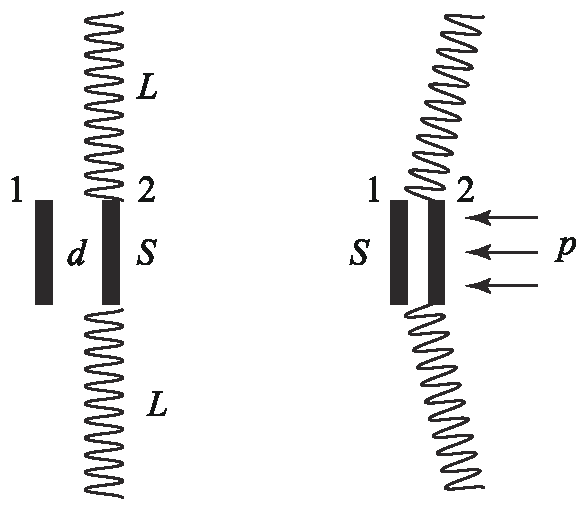
\includegraphics[width = 0.3\textwidth]{images/elec-problem-19.pdf} 
\end{flushright}

\tagged{student}{\vspace*{4cm}}
\begin{taggedblock}{teacher}

解析:
\end{taggedblock}
\end{example}
%%%%%%%%%%%%%%%%%%%%%%


\subsection{电容电路}
当在直流电路中接入电容器时,无论何种形式的电容器,例如平面平板电容器,其内部是由两个相对金属板构成,并不会形成通路,所以在分析线路内部的电流时电容可以当成断路来看待。
将来在学了交流电路以后以将会发现,虽然电容并没有直接的导线连接,但由于电磁场特有的规律,也能够导电。
虽然在直流电路中电容不导电,但接入线路中的电容也不是毫无反应,根据两端电压的不同,电容会被充电或放电。
例如下图所示的简单电路,当电容器$C$直接与一个电压为$U$的电源连接时,尽管回路中没有电流,但电容器的两极板将分别带有$Q=CU$的正负电荷。

同样的道理可以应用到多个电容共同存在的情况,当线路中有多个电容器时,有时可以将它们的效果看成是由一个给定容值的电容器,称为多个电容的等效电容。
和多个电阻的情况相类比,根据连接方式的不同,电容器之间也有并联、串联等简单的连接以及更复杂的情况。

简单的分析可知,两个并联的电容器两端的电压$U$相同,如果两个电容的容值分别为$C_1$、$C_2$的话,根据电容的基本关系,两电容器分别带有$Q_{1,2} = C_{1,2}U$的电量,这样总得来看则带了$Q=Q_1+Q_2$的电量,此时的等效电容
\begin{equation}
C = \frac{Q}{U} = \frac{Q_1+Q_2}{U} = C_1+C_2,
\end{equation}
很明显对于多个并联的电容电述关系同样成立,也就是说多个电容并联的等效电容是各个电容之和。
而对于如图所示两个电容的串联电路,电容器1的右侧极板和电容器2的左侧极板处于彼此连通但与其它部分隔绝的状态,根据电荷守恒它们两板带电量之和必需为零,所以当两个、或多个电容串联时各个电容器所带电量必然相同。
设带电量为$Q$,每个电容两板之间的电压则是$U_{1,2} = \frac{Q}{C_{1,2}}$,
简单的代数计算表明串联电容电路的等效电容
\begin{equation}
\frac{1}{C} = \frac{1}{C_1}+\frac{1}{C_2},  
\end{equation}
对于多个电容的串联,只需将上面公式稍加推广即可。
而那些无法看成多个电容串、并联的复杂电容网络则需要通过电容的性质和电路的特点,利用电荷守恒进行综合的判断。




%%%%%%%%%%%%%%%%%
\begin{example}

三个完全相同的电容器连接如图所示,已经电容器1带电量为$Q$,上板带正电荷jn容器2、3原来不带电。

1. 用导线将$a,b$相连,求电容器2的上、下板所带电量及其符号;

2.然后断开$a,b$,将$a,c$相连,再断开$a,c$,将$a,b$相连,求电容器2的上、下板所带电量及其符号;

3. 在上一问的情况下将$a,d$相连,再求电容器2上、下板所带电量及其符号。
\begin{flushright}
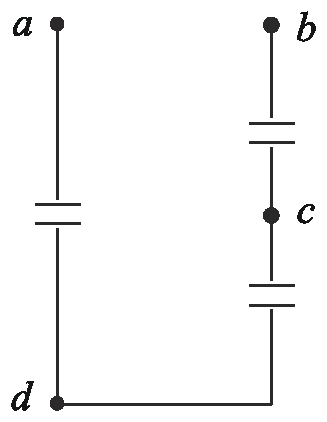
\includegraphics[width = 0.2\textwidth]{images/elec-problem-15.pdf} 
\end{flushright}
\tagged{student}{\vspace*{2cm}}
\begin{taggedblock}{teacher}

解析:
\end{taggedblock}
\end{example}
%%%%%%%%%%%%%%%%%%%%%%


%%%%%%%%%%%%%%%%%
\begin{example}
有如图所示的电容网格,电容的电位是$\mu\text{F}$,求$A、B$间的等效电容$C_{AB}$。
\begin{flushright}
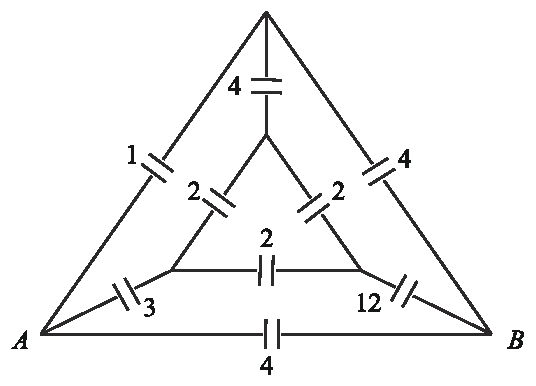
\includegraphics[width = 0.4\textwidth]{images/elec-problem-17.pdf} 
\end{flushright}

\tagged{student}{\vspace*{4cm}}
\begin{taggedblock}{teacher}

解析:
\end{taggedblock}
\end{example}
%%%%%%%%%%%%%%%%%%%%%%


%%%%%%%%%%%%%%%%%
\begin{example}
图所示电路中,电池的电动势为$\mathcal{E}$,两个电容器的电容皆为$C$,$K$为一单刀双掷开关。
开始时两电容器均不带电

1.第一种情况,现将$K$与$a$接通,达到稳定,此过程中电池内阻消耗的电能等于\kong\kong;再将$K$与$a$断开而与$b$接通,此过程中电池供给的电能等于\kong\kong。

2.第二种情况,现将$K$与$b$接通,达到稳定,此过程中电池内阻消耗的电能等于\kong\kong;再将$K$与$b$断开而与$a$接通,此过程中电池供给的电能等于\kong\kong。
\begin{flushright}
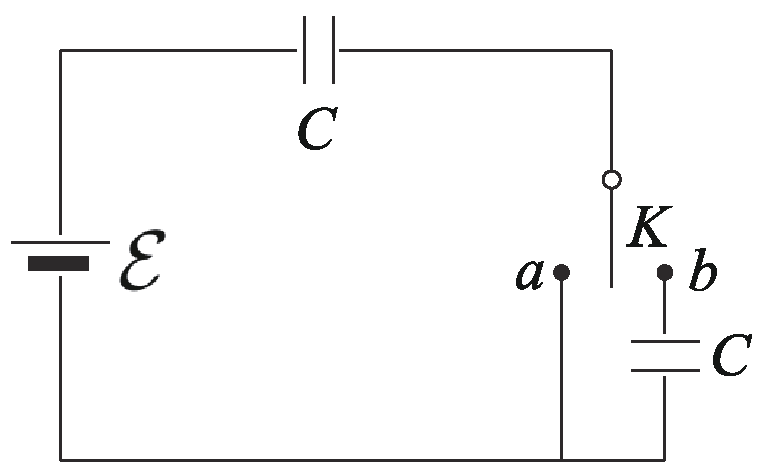
\includegraphics[width = 0.3\textwidth]{images/elec-problem-18.pdf} 
\end{flushright}


\tagged{student}{\vspace*{0cm}}
\begin{taggedblock}{teacher}

解析:
\end{taggedblock}
\end{example}
%%%%%%%%%%%%%%%%%%%%%%


\subsection{绝缘体、电介质与极化}

\emph{绝缘体}是指那些导电能力很弱的的物体,电磁学中将其又称之为\emph{电介质}。
导体之所以能够导电是因为内部存在大量可以自由移动的电荷能够在外电场作用下定向运动,和导体不同的是构成绝缘体的分子中正负电荷之间的束缚很大,在通常条件下不能够相互分离,所以在外电场作用下电荷无法运动。
取而代之的是在外电场作用下,构成绝缘体的分子中正负电荷会稍稍分开,形成一个电偶极子,其方向与外电场方向一致。
这个现象称为电介质的\emph{极化},宏观上看处于外电场中的电介质会在表面聚集一定的极化电荷。

根据电介质极化微观机制的不同,可将电介质分为两大类。
第一类电介质的分子当无外场存在时正负电荷“中心”是重合的,这类分子称为无极分子,外场的作用像是将无极性分子的正负电荷“拉开”形成电偶极子。
另一类电介质分子本身正负电荷就是分开的,称为极性分子,已经形成一个电偶极子,无外电场时这些电偶极子的指向杂乱无章,并不显示电效应,但当外电场存在时它们在一定程度上将有序排列。
不同的电介质对外电场的响应,或极化不尽相同,为了描述这种不同,我们引入一个新的物理量称为\emph{介电常数},当在真空中为$C_0$的电容器中充满某种电介质时,它的电容将发生变化,一般来说变为原先的$\varepsilon_r$倍
\begin{equation}
C = \varepsilon_r C_0
\end{equation}
将$\varepsilon_r$称为该介质的\emph{相对介电常数},它与真空的介电常数$\varepsilon_0$的乘积称为电介质的介电常数,一般用$\varepsilon$表示。
例如对于充满介电常数为$\varepsilon$、极板面积为$S$、两板相距$d$平行板电容器的电容
\begin{equation}
C = \varepsilon\frac{S}{d} = \varepsilon_r\varepsilon_0\frac{S}{d}.
\end{equation}


%%%%%%%%%%%%%%%%%
\begin{example}
空间中

\tagged{student}{\vspace*{4cm}}
\begin{taggedblock}{teacher}

解析:
\end{taggedblock}
\end{example}
%%%%%%%%%%%%%%%%%%%%%%

%%%%%%%%%%%%%%%%%
\begin{example}

原先电容器的电容为$C_0$,现插入厚度为$\frac{d}{2}$,介电常数为$\varepsilon$的介质,且只占$\frac{S}{2}$的面积,在忽略边缘效应的情况下求现在电容器的电容量$C$。
\begin{flushright}
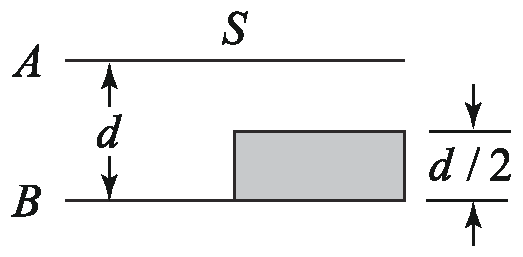
\includegraphics[width = 0.3\textwidth]{images/elec-problem-20.pdf} 
\end{flushright}
\tagged{student}{\vspace*{2cm}}
\begin{taggedblock}{teacher}

解析:
\end{taggedblock}
\end{example}
%%%%%%%%%%%%%%%%%%%%%%


%%%%%%%%%%%%%%%%%
\begin{example}

如图所示,一平行板电容器,极板面积为$S$,其上半部为真空,而下半部充满相对介电常数为$\varepsilon_r$的均匀电介质,当两极板分别带上$+Q$和$−Q$的电量后,忽略边缘效应的情况下试求:

1. 板上自由电荷分布;

2. 两板之间的场强;

3. 介质表面的极化电荷。
\begin{flushright}
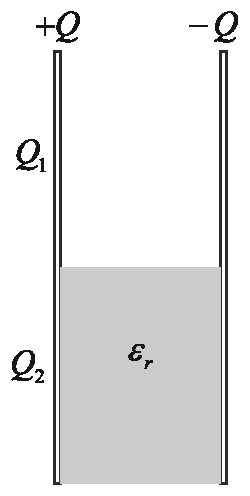
\includegraphics[width = 0.2\textwidth]{images/elec-problem-21.pdf} 
\end{flushright}

\tagged{student}{\vspace*{4cm}}
\begin{taggedblock}{teacher}

解析:
\end{taggedblock}
\end{example}
%%%%%%%%%%%%%%%%%%%%%%